\sloppy\section{K10 -- Optyczne nośniki informacji}

Dyski optyczne zaliczają się do nośników informacji. Zostały wprowadzone jako alternatywa dla dysków magnetycznych. Odczyt danych z dysku optycznego odbywa się za pomocą wiązki światła (a konkretniej promienia lasera) -- nazwa opiera się na zasadzie działania takiego nośnika.

W dzisiejszych czasach nośniki optyczne mają różne pojemności, stosowane są w różnych dziedzinach (np. na nich dystrybuowana jest muzyka, czy też filmy). 

Do dysków optycznych zaliczamy:

\textbf{LaserDisc} -- analogowy dysk optyczny, który miał 30 cm średnicy, składał się z dwóch jednostronnych aluminiowych dysków pokrytych plastikiem. Na nośniku był zapisywany analogowy sygnał wideo cyfrowy analogowy i/lub cyfrowy sygnał dźwiękowy. Posiadał formaty kodowania:
\begin{itemize}
\item CAV -- stała prędkość kątowa, dyski pracowały ze stałą prędkością kątową 1800rpm, z odczytem jednej klatki na obrót, pojemność wynosiła 30 min na stronę, CAV posiadała funkcje stop klatki, zmiany prędkości odtwarzania oraz cofanie,
\item CLV -- stała prędkość liniowa, nie posiada funkcji z CAV, przez zmniejszenie prędkości obrotowej zwiększyła się pojemność do 60 min obrazu lub dźwięku,
\item CAA (wariant CLV) -- stałe przyspieszenie kątowe, wynalezione by wyeliminować zjawisko wchodzenia jednego kanału na drugi z CLV, różnica między CAA a CLV polega na dopasowaniu kąta obrotu dysku, zamiast stopniowego liniowego zwalniania, dzięki CAA znacznie poprawiła się jakość obrazu na nośniku,
\end{itemize}

\textbf{CompactDisk} -- początkowo był stworzony tylko do przechowywania muzyki, później dodano możliwość przechowywania danych. Płyta CD ma średnicę 12 cm i może pomieścić do 80 min dźwięku lub 700 MB danych. Istnieje również format mini-CD, jednak jest on mniej popularny (do 24 min dźwięku, 210 MB pojemności; inny format -- ,,wizytówka'' CD -- do 6 min dźwięku, do 65 MB pojemności). Formaty CD:
\begin{itemize}
\item Audio-CD -- format to dwukanałowy 16-bitowy PCM, z próbkowaniem 44.1 kHz na kanał, dźwięk mono nie występuje w implementacji, zazwyczaj dźwięk mono jest przedstawiony jako dwa takie same kanały w stereo. CD-Text jest rozszerzeniem Audio-CD, zezwala na zachowanie informacji tekstowych (np. nazwa albumu, artysty, ścieżek).
\item Video-CD -- cyfrowy standard do przechowywania wideo na płytach CD. W porównaniu z kasetami VHS jakość wideo nie pogarsza się po każdym użyciu. Wykorzystywane rozdzielczości to 352x240 oraz 352x288.
\item CD-R -- płyta może zostać raz zapisana, posiada warstwę barwnika, który jest stapiany przy zapisywaniu,
\item CD-RW -- płyta do zapisu wielokrotnego, kasowanie danych odbywa się za pomocą lasera (następuje topnienie stopu, traci swoją strukturę polikrystaliczną).
\end{itemize}

\textbf{DVD} -- medium do przechowywania różnego typu danych, zazwyczaj do oprogramowania oraz filmów. Nośniki posiadają takie same wymiary jak płyty CD, jednak można na nich zapisać więcej danych. Zwiększenie danych jest możliwe dzięki zwiększeniu gęstości zapisu danych (użyto lasera o krótszej długości fali). Powstały również płyty dwustronne oraz dwuwarstwowe. Podobnie jak w przypadku płyt CD, istnieją tutaj płyty jednokrotnego oraz wielokrotnego zapisu. W przeciwieństwie do CD, płyty DVD muszą zawierać system plików. Płyty DVD również posiadają formaty Audio oraz Video. Płyty audio posiadają dużą możliwość konfiguracji kanałów, z różnym próbkowaniem (nawet do 24-bit, 192 kHz). W porównaniu do CD-Audio pozwala zapisać więcej dźwięku w lepszej jakości. Zapis wideo na płytach DVD-Video wykorzystuje kodek MPEG-2. Najczęściej stosowane rozdzielczości to 720x576 oraz 720x480. Następcą DVD jest HD DVD, który zawierał gęstszy zapis danych, jednakże został porzucony na rzecz płyt Blu-Ray (wykorzystują tę samą długość fali lasera).

Dostęp do drugiej warstwy możliwy jest przez przepuszczenie lasera przez pierwszą, częściowo przepuszczalną warstwę. Zmiana ścieżki może potrwać kilka sekund, przez co może spowodować chwilowe zatrzymanie pracy napędu.

\textbf{Blu-ray} jest kolejnym formatem dysków optycznych. Dyski posiadają 25 GB na warstwę, przy zapisie dwu-warstwowym daje to 50 GB. W 2008 roku przedstawiono szesnasto-warstwową płytę BD, o pojemności 400 GB. Istnieją również formaty trzy- i cztero-warstwowe płyt BD. Nazwa technologii wywodzi się od koloru wykorzystywanego lasera. 

\begin{figure}[H]
\caption{Porównanie formatów płyt. Źródło: Wikipedia}
\centering
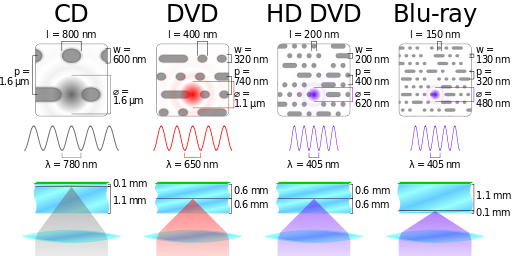
\includegraphics[width=\linewidth]{K10_Porownanie_plyt_Wikipedia.png}
\end{figure}

\textbf{HVD} (Holographic Versatile Disc) -- technologia dysków optycznej nowej generacji, teoretycznie pozwala pomieścić do 6 TB na jednej warstwie. Zapis danych odbywa się w trójwymiarowej przestrzeni dysku. Wykorzystywane są dwa lasery -- zielony oraz czerwony.

Stany logiczne na płycie CD są reprezentowane przez pity (wgłębienia, reprezentują 0) oraz landy (przerwy między wgłębieniami, reprezentują 1). Gdy wiązka trafia na land, to jest rozpraszana i nie wraca do czytnika. Przy picie wiązka jest odbijana i trafia z powrotem do czujnika. Dane zapisywane są od środka na zewnątrz płyty.

Kodowanie wykorzystywane w płytach to EFM (eight to fourteen modulation). Jest wykorzystywane ze względu na ograniczenia technologiczne (szybkości światła i odpowiedzi modulatora). Przez to długości pitów i landów muszą znajdować się w przedziale od 3 do 11 bitów kanałowych (ciąg kilku pitów/landów nie może być krótszy niż 3 bity kanałowe oraz dłuższy niż 11). Dlatego każde 8 bitów jest zapisywane za pomocą 14 bitów kanałowych. Do konwersji jest wykorzystywana tabela, która jest zapisana w firmware napędu. 

Dla płyt DVD, ze względu na mniejsze odległości stosowany jest zapis bajtów na 16 bitowych sekwencjach. Długości pitów i landów muszą być w przedziale od 3 do 14 bitów kanałowych.

Płyty Blu-ray wykorzystują kodowanie podobne do EFM, 17PP (one seven parity preserving). Wykorzystuje kodowanie, w którym każde 2 bity są zapisywane na 3 bitach, a samo kodowanie odbywa się w grupach po 2 albo 4 bity. Dodatkowo występują bity kontrolne (DC), po których wystąpieniu (jeśli DC == 1), zmieniana jest polaryzacja strumienia NRZI.

NRZI -- metoda odwzorowania sygnału binarnego, bez powrotów do zera. Wykorzystuje dwa stany logiczne. Przejście między nimi następuje, gdy transmitowany bit wynosi 1, w przypadku bitu 0 zmiana nie następuje.